\chapter{TINJAUAN PUSTAKA}
\label{chap:tinjauanpustaka}


\section{Hasil penelitian/perancangan terdahulu}
\label{Hasil penelitian/perancangan terdahulu}
Dalam tesis yang dilakukan oleh Thilderkvist dan Svensson,
platform \emph{PhantomX Hexapod Mark II} digunakan sebagai basis robot. Robot
ini memiliki rangka berbahan aluminium dan dilengkapi dengan total delapan belas
\emph{servo motor}—tiga buah pada setiap kaki—yang memungkinkan gerakan dalam
tiga derajat kebebasan (\emph{3-DOF}) per kaki. Setiap sendi dikendalikan secara
independen menggunakan aktuator servo tipe \emph{AX-12A} dari Dynamixel, yang
terkenal akan presisi dan torsi yang tinggi. Di bagian pusat tubuh robot,
dipasang sebuah mikrokontroler utama yang bertugas untuk mengeksekusi algoritma
kendali gerak yang telah dikembangkan di lingkungan \emph{MATLAB/Simulink}.
Selain itu, sistem dilengkapi dengan sensor \emph{IMU} (Inertial Measurement
Unit) untuk mendeteksi orientasi dan kemiringan tubuh, yang sangat penting dalam
menjaga keseimbangan saat robot bergerak di permukaan yang tidak rata
\parencite{Thilderkvist2015}.

Pada penelitian yang dilakukan Xinan Wang dkk berfokus pada analisis kinematika robot 
lengan humanoid dengan enam derajat kebebasan (6-DOF). Dalam studi tersebut, model 
\emph{forward kinematic} dibentuk menggunakan metode Denavit-Hartenberg (D-H), sementara solusi 
\emph{inverse kinematic} diselesaikan secara kombinasi antara metode numerik dan aljabar. 
Penelitian ini juga mengembangkan simulasi berbasis MATLAB untuk memverifikasi 
keakuratan solusi kinematika yang dihasilkan. Hasil verifikasi menunjukkan bahwa 
deviasi maksimum antara pose target dan aktual hanya sebesar 0.0009 radian pada sumbu 
roll, yang menunjukkan presisi tinggi dari model kinematika yang digunakan. Pendekatan 
ini menunjukkan efektivitas integrasi antara metode analitik dan numerik dalam 
menyelesaikan permasalahan kinematika lengan robot kompleks. \parencite{wang2024kinematics}

\sloppy
Penelitian yang dilakukan Dologa dkk memperkenalkan platform robot hexapod
biomimetik yang dirancang dengan fokus pada modularitas, efisiensi biaya, dan
kesederhanaan struktur kontrol. Penelitian ini mencakup tiga fase utama: desain
mekanik, pengembangan sistem elektronik, dan implementasi sistem kontrol
berbasis \emph{forward kinematic} serta \emph{inverse kinematic}. Robot memiliki 3 derajat
kebebasan per kaki dengan penggerak servo MG995 yang dikendalikan oleh
Arduino Mega 2560 dan dikomunikasikan melalui Bluetooth. Model \emph{inverse kinematic}
dikembangkan secara geometrik untuk memungkinkan gerakan spasial yang presisi.
Melalui simulasi dan implementasi nyata menggunakan bagian-bagian hasil cetak 3D,
platform ini terbukti mampu bergerak maju, mundur, dan berputar di titik tetap
dengan kestabilan yang baik, serta mampu menanggung beban tambahan. \parencite{10554226}

\section{Teori/Konsep Dasar}
\label{sec:konsep dasar}

\subsection{Robot \emph{Hexapod}}
Robot berkaki enam atau \emph{hexapod} adalah jenis robot yang konfigurasi kakinya terinspirasi
dari hewan-hewan berkaki enam seperti serangga atau laba-laba. Konfigruasi robot hexapod ini sangat
popler pada robot mobile karena stabilitasnya yang tinggi pada saat bergerak, sehingga mengurangi 
kompleksitas kontrol dan desain mekanik. \parencite{RobotHexapod}

\subsection{\emph{Forward Kinematic} dan \emph{Inverse Kinematic}}
\emph{Forward kinematic}  adalah metode yang digunakan untuk mengonversi nilai sudut pada 
setiap joint menjadi koordinat kartesian di titik ujung \emph{end-effector}. Dengan menggunakan 
metode ini, posisi dan orientasi \emph{end-effector} (dikenal sebagai robot pose) dapat dihitung 
berdasarkan konfigurasi sudut pada masing-masing \emph{joint} serta struktur mekanik dari robot 
tersebut.\parencite{ModernRobotics}

\begin{figure} [H] \centering
  % Nama dari file gambar yang diinputkan
  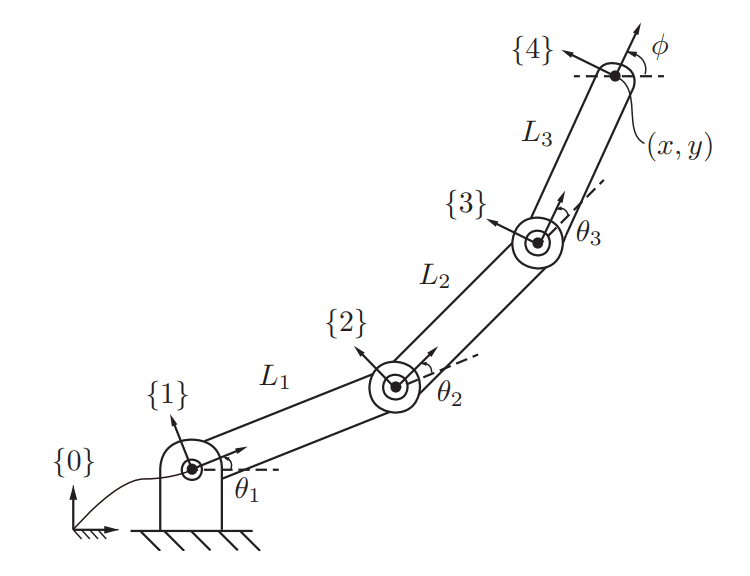
\includegraphics[scale=0.35]{gambar/Planar 3 DOF.png}
  % Keterangan gambar yang diinputkan
  \caption{Contoh lengan robot 3 DOF \parencite{ModernRobotics}}
  % Label referensi dari gambar yang diinputkan
  \label{fig:Planar3DOF}
\end{figure}

Dengan menggunakan \emph{forward kinematic} pada robot lengan 3 DOF seperti pada Gambar \ref{fig:Planar3DOF},
dapat diperoleh persamaan posisi \emph{end-effector} sebagai berikut:

\begin{equation}
  \label{eq:Forward Kinematic}
  \begin{aligned}
    x &= L_1 \cos \theta_1 + L_2 \cos(\theta_1 + \theta_2) + L_3 \cos(\theta_1 + \theta_2 + \theta_3), \\
    y &= L_1 \sin \theta_1 + L_2 \sin(\theta_1 + \theta_2) + L_3 \sin(\theta_1 + \theta_2 + \theta_3).
  \end{aligned}
\end{equation}
Jika lengan robot hanya membutuhkan posisi (x,y) dari \emph{end-effector}, ruang gerak
robot dianggap sebagai dua dimensi pada bidang x-y, maka \emph{forward kinematic} hanya
menggunakan persamaan \ref{eq:Forward Kinematic}. Namun jike orientasi dari \emph{end-effector}
dibutuhkan, maka diperlukan satu persamaan lagi untuk menghitung sudut orientasi

\begin{equation}
  \label{eq:end-effector}
  \phi = \theta_1 + \theta_2 + \theta_3.
\end{equation}

\emph{Inverse kinematic} adalah metode yang digunakan untuk menghitung sudut pada setiap
\emph{joint} berdasarkan posisi dan orientasi yang diinginkan dari \emph{end-effector}.
Posisi dan orientasi dari \emph{end-effector} yang diinginkan harus sesuai dengan kemampuan
struktur mekanik yang ada. Untuk menyelesaikan \emph{inverse kinematic} pada sebuah robot,
terdapat beberapa kemungkinan solusi yang dapat dihasilkan.\parencite{inverseKinematics}

% \begin{figure} [H] \centering
%   % Nama dari file gambar yang diinputkan
%   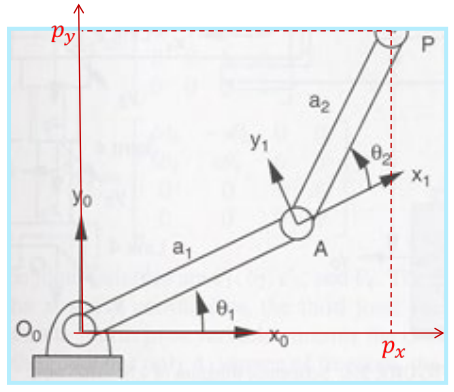
\includegraphics[scale=0.65]{gambar/Planar 2 DOF.png}
%   % Keterangan gambar yang diinputkan
%   \caption{Lengan Robot 2 DOF \parencite{inverseKinematics}}
%   % Label referensi dari gambar yang diinputkan
%   \label{fig:Planar2DOF}
% \end{figure}

Terdapat dua pendekatan \emph{inverse kinematic} yang
dapat digunakan untuk menghitung sudut dari setiap \emph{joint} berdasarkan posisi dari
\emph{end-effector} yang diinginkan.  

\begin{figure}[H]
  \centering
  \begin{subfigure}{0.45\textwidth}
    \centering
    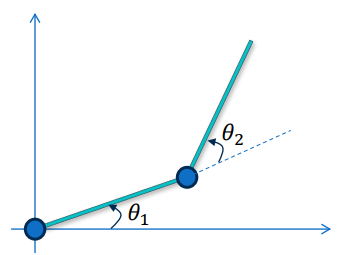
\includegraphics[width=\textwidth]{gambar/ElbowDown.png}
    \caption{Elbow Down}
    \label{fig:ElbowDown}
  \end{subfigure}
  \hfill
  \begin{subfigure}{0.45\textwidth}
    \centering
    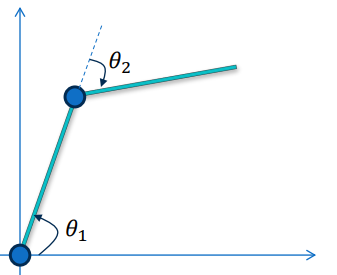
\includegraphics[width=\textwidth]{gambar/ElbowUp.png}
    \caption{Elbow Up}
    \label{fig:ElbowUp}
  \end{subfigure}
  \caption{Pendekatan elbow down dan elbow up \parencite{inverseKinematics}}
  \label{fig:TwoImages}
\end{figure}
Untuk pendekatan elbow down, dapat digunakan aturan cos untuk menggunakan aturan cosinus
untuk mencari nilai $\theta_2$ sebagai berikut : 

\begin{equation}
  \label{eq:ElbowDownTheta2}
  \begin{aligned}
    (O_O P)^2 & = (O_O A_1)^2 + (A_1 P)^2 - 2(O_O A_1)(A_1 P)\cos(\pi - \theta_2), \\
    p_x^2 + p_y^2 & = a_1^2 + a_2^2 + 2a_1a_2\cos\theta_2, \\
    \theta_2 & = \cos^{-1}\left(\frac{p_x^2 + p_y^2 - a_1^2 - a_2^2}{2a_1a_2}\right).
  \end{aligned}
\end{equation}
Kemudian untuk mendapatkan $theta_1$ dapat didapatkan dengan mengurangkan sudut yang
dihasilkan oleh $p_x$ dan $p_y$ dengan sudut yang dihasilkan oleh $\theta_2$.
\begin{equation}
  \label{eq ElbowDownTheta1}
  \theta_1 = \tan^{-1}\left(\frac{p_y}{p_x}\right) - \tan^{-1}\left(\frac{a_2\sin\theta_2}{a_1 + a_2\cos\theta_2}\right).
\end{equation}
Pendekatan elbow up juga menggunakan aturan cosinus untuk mencari nilai $\theta_2$ sedangkan
untuk mencari nilai $\theta_1$ sama dengan pendekatan elbow down. 
\begin{equation}
  \label{eq:ElbowUpTheta2}
  \begin{aligned}
    \theta_2 & = -\cos^{-1}\left(\frac{p_x^2 + p_y^2 - a_1^2 - a_2^2}{-2a_1a_2}\right),\\
    \theta_1 & = \tan^{-1}\left(\frac{p_y}{p_x}\right) - \tan^{-1}\left(\frac{a_2\sin\theta_2}{a_1 + a_2\cos\theta_2}\right).
  \end{aligned} 
\end{equation}
Kedua pendekatan ini merupakan solusi dari \emph{inverse kinematic} yang dapat digunakan
untuk menghitung sudut dari setiap \emph{joint} berdasarkan posisi dari \emph{end-effector}
yang diinginkan. Namun, kedua pendekatan ini tidak dapat digunakan untuk semua tipe robot.
Ketika jumlah \emph{joint} bertambah, maka solusi dari \emph{inverse kinematic} juga akan
berbeda-beda.

\subsection{\emph{Trajectoty Planning}}
Selama pergerakan robot, kontroller robot diberikan serangkaian posisi dan kecepatan tujuan 
secara terus-menerus untuk diikuti. Posisi robot sebagai fungsi waktu ini disebut
sebagai trajektori. Dalam beberapa kasus, trajektori sepenuhnya ditentukan oleh tugas yang 
harus dilakukan – misalnya, \emph{end-effector} mungkin perlu mengikuti objek bergerak yang 
sudah diketahui. Namun, dalam kasus lain, seperti ketika robot hanya berpindah dari satu 
posisi ke posisi lain dalam waktu tertentu, terdapat kebebasan untuk merancang 
trajektori yang memenuhi batasan tersebut. Proses merancang lintasan  ini disebut 
\emph{trajectory planning}. Trajektori yang dirancang harus berupa fungsi waktu
yang halus (smooth) dan tetap mematuhi batasan sistem, seperti batas kecepatan,
percepatan, atau torsi maksimum pada setiap joint robot. Tujuan akhirnya adalah
menghasilkan gerakan yang efisien, stabil, dan aman bagi sistem maupun
lingkungannya. \parencite{ModernRobotics}

Untuk mencapai tujuan ini, terdapat beberapa metode perencanaan trajektori yang umum digunakan.
Salah satu metode yang umum digunakan adalah metode interpolasi linear. Interpolasi linier
bertujuan untuk mendapatkan fungsi linier yang menghubungkan dua titik pada suatu garis.
\parencite{LinierInterpolation}

\begin{figure} [H] \centering
  % Nama dari file gambar yang diinputkan
  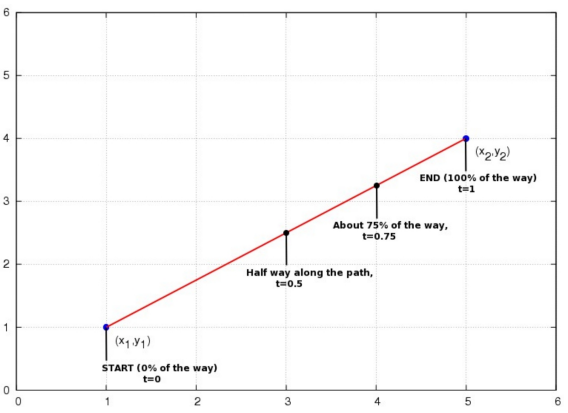
\includegraphics[scale=0.65]{gambar/Interpolasi Linier.png}
  % Keterangan gambar yang diinputkan
  \caption{Hubungan antara dua titik sepanjang sebuah garis lurus \parencite{LinierInterpolation}}
  % Label referensi dari gambar yang diinputkan
  \label{fig:InterpolasiLinier}
\end{figure}

Pada gambar \ref{fig:InterpolasiLinier} terdapat dua titik yang terhubung oleh garis lurus. (x1,y1)
merupakan titik awal dan (x2,y2) merupakan titik akhir. Untuk mendapatkan fungsi linier
yang memberikan posisi pada garis lurus antara dua titik tersebut pada satu waktu tertentu, dapat digunakan
persamaan berikut: 
\begin{equation}
  \label{eq:InterpolasiLinier}
  x(t) = x_1 + (x_2 - x_1)t, \quad y(t) = y_1 + (y_2 - y_1)t, \quad 0 \leq t \leq 1.
\end{equation}
Hasil interpolasi linier ini dapat digunakan sebagai input untuk \emph{inverse kinematic}
agar dapat menghasilkan sudut dari setiap \emph{joint} berdasarkan posisi dari
\emph{end-effector} yang diinginkan.

\subsection{Polah Langkah/\emph{Gait}}
Pola pergerakan kaki yang digunakan untuk berjalan atau berlari disebut sebagai
\emph{gait}, dan memiliki peran penting dalam menentukan desain sistem tungkai robot.
Desain fisik robot sangat dipengaruhi oleh jenis gait yang akan diterapkan.
Untuk mendukung pola langkah statis, robot dirancang dengan postur tubuh
yang melebar dan merentang guna memaksimalkan stabilitas selama pergerakan.
Sebaliknya, untuk pola langkah dinamis, robot biasanya memiliki postur tubuh
yang lebih tegak dengan pusat massa yang lebih tinggi, sehingga dapat
memperpanjang konstanta waktu jatuh dan mendukung gerakan yang lebih cepat dan
lincah. \parencite{GaitRobot}

Pada gerakan robot \emph{hexapod}, pergerakan setiap kaki dibagi menjadi dua fase utama:
\begin{itemize} 
  \item Fase dukungan (\emph{support phase}): Pada fase ini, kaki
menyentuh tanah dan memberikan dukungan pada tubuh robot. Selama fase ini, kaki
tidak bergerak. 
\item Fase ayunan (\emph{swing phase}): Pada fase ini, kaki
terangkat dari tanah dan bergerak menuju posisi baru sebelum kembali menyentuh
tanah. Selama fase ini, kaki bergerak tanpa memberikan dukungan pada tubuh robot.
\parencite{GaitSwingSupport} 
\end{itemize}

Robot \emph{hexapod} memiliki enam kaki, sehingga terdapat beberapa algoritma pola langkah
yang umum digunakan, antara lain:
\begin{itemize} 
  \item \emph{Tripod gait}: Pada pola langkah ini, tiga kaki
bergerak secara bersamaan sementara tiga kaki lainnya tetap di tanah. Pola
langkah ini memberikan stabilitas yang baik dan memungkinkan robot bergerak
dengan kecepatan sedang. 
\item \emph{Wave gait}: Pada pola langkah ini, kaki
bergerak secara bergantian dalam urutan tertentu, mirip dengan gelombang. Pola
langkah ini memberikan stabilitas yang baik tetapi cenderung lebih lambat
dibandingkan dengan pola langkah tripod. 
\item \emph{Ripple gait}: Pada pola
Dua atau tiga kaki bergerak secara bergantian, namun tidak serempak seperti tripod gait. 
\parencite{GaitAlgorithm}
\end{itemize}

\begin{figure} [H] \centering
  % Nama dari file gambar yang diinputkan
  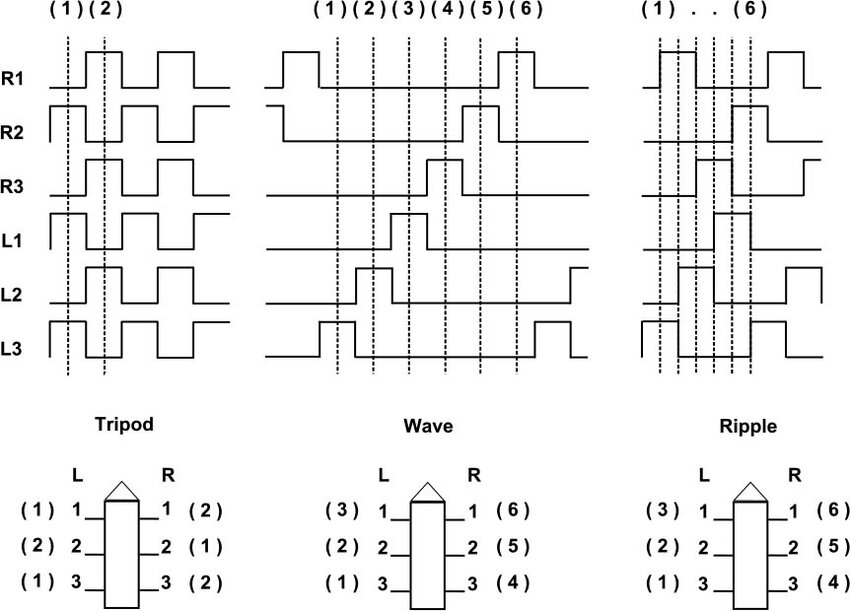
\includegraphics[scale=1.5]{gambar/gait.png}
  % Keterangan gambar yang diinputkan
  \caption{algoritma pola langkah robot \emph{hexapod}\parencite{GaitAlgorithm}}
  % Label referensi dari gambar yang diinputkan
  \label{fig:GaitHexapod}
\end{figure}

Pemilihan jenis gait ini bergantung pada kebutuhan spesifik aplikasi, seperti
tuntutan stabilitas, kecepatan, efisiensi energi, dan medan operasional robot

\subsection{\emph{Dynamixel Protocol 1.0}}
\emph{Dynamixel Protocol 1.0} adalah protokol komunikasi yang digunakan oleh
servo motor \emph{Dynamixel} untuk berkomunikasi dengan mikrokontroler atau
perangkat lain. Mikrokontroler dan servo berkomunikasi satu sama lain (dua arah)
dengan mengirimkan dan menerima data dalam bentuk paket. Paket dibagi menjadi dua
bagian, yaitu : 
\begin{itemize}
  \item \emph{Instruction Packet}: Paket yang dikirimkan oleh mikrokontroler. Paket ini
  berisi instruksi yang akan dieksekusi oleh servo. 
  \item \emph{Status Packet}: Paket yang dikirimkan oleh servo. Paket ini mengembalikan
  informasi status dari servo setelah menerima instruksi dari mikrokontroler. 
\end{itemize}  
\begin{table}[H]
  \centering
  \caption{Struktur \emph{Instruction Packet} data Dynamixel Protocol 1.0}
  \label{tab:DynamixelPacket}
  \renewcommand{\arraystretch}{1.5}
  \begin{tabular}{|c|c|c|c|c|c|c|c|c|}
    \hline
    \textbf{H1} & \textbf{H2} & \textbf{ID} & \textbf{LEN} & \textbf{INST} & \textbf{P1} & \textbf{$\cdots$} & \textbf{PN} & \textbf{CHKSUM} \\
    \hline
    0xFF & 0xFF & Servo ID & Length & Instruction & Param 1 & $\cdots$ & Param N & Checksum \\
    \hline
  \end{tabular}
\end{table}
Dimana maksud dari masing-masing kolom adalah sebagai berikut:
\begin{itemize}
  \item \textbf{H1} dan \textbf{H2}: Header dari paket yang menunjukkan bahwa ini adalah
  paket \emph{Dynamixel}. Nilai header adalah 0xFF.
  \item \textbf{ID}: ID dari servo yang akan dikontrol. Total ID servo yang dapat digunakan
  adalah ID 0 hingga ID 253. Terdapat juga ID broadcast yaitu ID 254 yang digunakan
  untuk mengirimkan instruksi ke semua servo yang terhubung dalam satu bus.
  \item \textbf{LEN}: Panjang dari paket data, termasuk instruksi dan parameter. Lenght 
  dihitung dari banyak parameter + 2.
  \item \textbf{INST}: Instruksi yang akan dieksekusi oleh servo. Tabel \ref{tab:Instruction}
  menunjukkan instruksi yang digunakan dalam \emph{Dynamixel Protocol 1.0}.
  \item \textbf{P1} hingga \textbf{PN}: Parameter merupakan data dari instruksi yang dikirimkan. 
  Setiap instruksi memiliki jumlah parameter yang berbeda-beda. 
  \item \textbf{CHKSUM}: \emph{Checksum} adalah nilai yang digunakan untuk memverifikasi
  data yang dikirimkan. Nilai  \emph{checksum} dihitung dengan menggunakna formula sebagai 
  berikut:
  \begin{equation}
    \label{eq:Checksum}
    CHKSUM = \sim ( ID + Length + Instruction + Parameter1 + \ldots + Parameter N )
  \end{equation}
  Operator "$\sim$" \emph{bitwise NOT} digunakan untuk membalikkan semua bit dari hasil penjumlahan.
  Ketika nilai perhitungan \emph{checksum} lebih dari 255, maka hanya \emph{lower byte} yang digunakan.
\end{itemize}
\begin{table}[H]
\centering
\caption{Instruksi \emph{Dynamixel Protocol 1.0}}
\label{tab:Instruction}
\begin{tabular}{|c|l|p{8cm}|}
\hline
\textbf{Value} & \textbf{Instruksi} & \textbf{Deskripsi} \\
\hline
0x01 & Ping & Instruksi untuk memeriksa apakah paket telah sampai ke perangkat dengan ID yang sama seperti ID dalam paket. \\
\hline
0x02 & Read & Instruksi untuk membaca data dari perangkat. \\
\hline
0x03 & Write & Instruksi untuk menulis data ke perangkat. \\
\hline
0x04 & Reg Write & Instruksi untuk mendaftarkan paket instruksi ke status siaga; paket akan dieksekusi kemudian melalui instruksi Action. \\
\hline
0x05 & Action & Instruksi untuk mengeksekusi paket yang telah dikirimkan menggunakan Reg Write. \\
\hline
0x06 & Factory Reset & Instruksi untuk mengatur ulang Tabel Kontrol ke pengaturan awal pabrik. \\
\hline
0x08 & Reboot & Instruksi untuk memulai ulang DYNAMIXEL (Lihat produk yang didukung dalam deskripsi). \\
\hline
0x83 & Sync Write & Instruksi untuk menulis data pada beberapa servo secara bersamaan. \\
\hline
0x92 & Bulk Read & Instruksi untuk membaca data dari servo secara bersamaan. \\
\hline
\end{tabular}
\end{table}

Setelah \emph{Instruction Packet} dikirimkan, servo akan memproses instruksi tersebut
dan mengirimkan \emph{Status Packet} sebagai balasan. Tabel \ref{tab:StatusPacket}
menunjukkan struktur dari \emph{Status Packet} yang dikirimkan oleh servo.
\begin{table}[H]
\centering
\caption{Struktur \emph{Status Packet} data Dynamixel Protocol 1.0}
\label{tab:StatusPacket}
\renewcommand{\arraystretch}{1.5}
\begin{tabular}{|c|c|c|c|c|c|c|c|c|}
  \hline
  \textbf{H1} & \textbf{H2} & \textbf{ID} & \textbf{LEN} & \textbf{Error} & \textbf{P1} & \textbf{$\cdots$} & \textbf{PN} & \textbf{CHKSUM} \\
  \hline
  0xFF & 0xFF & Servo ID & Length & Error & Param 1 & $\cdots$ & Param N & Checksum \\
  \hline
\end{tabular}
\end{table}

Yang membedakan \emph{Status Packet} dengan \emph{Instruction Packet} adalah 
pada paket kelima. Pada \emph{Status Packet} paket kelima adalah \emph{Error} 
yang menunjukkan apakah terjadi error pada servo. Tabel \ref{tab:Error} 
menujkan error yang mungkin terjadi pada servo. 

\begin{table}[H]
\centering
\caption{Tabel Error Bit Dynamixel}
\label{tab:Error}
\begin{tabular}{|c|l|p{9cm}|}
\hline
\textbf{Bit} & \textbf{Error} & \textbf{Deskripsi} \\
\hline
Bit 7 & 0 & - \\
\hline
Bit 6 & Instruction Error & Jika instruksi yang tidak dikenal dikirim atau instruksi aksi dikirim tanpa instruksi Reg Write, bit ini akan diset menjadi 1. \\
\hline
Bit 5 & Overload Error & Jika beban saat ini tidak dapat dikendalikan oleh torsi yang telah diatur, bit ini akan diset menjadi 1. \\
\hline
Bit 4 & Checksum Error & Jika checksum dari paket instruksi yang dikirim salah, bit ini akan diset menjadi 1. \\
\hline
Bit 3 & Range Error & Jika suatu instruksi berada di luar jangkauan penggunaan yang diizinkan, bit ini akan diset menjadi 1. \\
\hline
Bit 2 & Overheating Error & Jika suhu internal DYNAMIXEL melebihi batas suhu operasi yang ditentukan di tabel kontrol, bit ini akan diset menjadi 1. \\
\hline
Bit 1 & Angle Limit Error & Jika Goal Position berada di luar rentang dari batas sudut CW ke batas sudut CCW, bit ini akan diset menjadi 1. \\
\hline
Bit 0 & Input Voltage Error & Jika tegangan yang diterapkan berada di luar rentang tegangan operasi yang ditentukan di tabel kontrol, bit ini akan diset menjadi 1. \\
\hline
\end{tabular}
\end{table}

Paket error terdiri dari 8 bit, yang masing-masing menunjukkan error yang
mungkin terjadi pada servo. Sebagai contoh, jika paket error bernilai 0x24 (dalam biner 00100100), maka
error yang terjadi adalah \emph{Overload Error} dan \emph{Overheating Error}.